\documentclass[12pt]{article}

\usepackage{amsmath}
\usepackage{amssymb}
\usepackage{amsfonts}
\usepackage[style=iso]{datetime2}
\usepackage{graphicx}
\usepackage{float}

\graphicspath{ {./Images/} }


\begin{titlepage}
\title{Calculus I: Review of Inverse Functions}
\author{The Melon Man}
\date{\today}
\end{titlepage}

\renewcommand{\thesection}{\Roman{section}}

\allowdisplaybreaks

\setlength{\parindent}{0pt}
\setlength{\parskip}{1em}

\begin{document}
\maketitle

If we have a function $f(x)$ such that $f(x)=x^2$, we may want to find the inverse of this function.
We denote the inverse of some function with the $-1$ before the opening parentheses.
For instance, the inverse of $f(x)$ would be $f^{-1}(x)$.
This should not be confused with raising the function to the $-1$th power, as that would give us something different.
This may be confusing, especially with the trigonometric functions who have well-known inverses as well as functions that equal them raised to the $-1$th power.

Taking the inverse of a function after taking the function may be thought of reversing what the function did and giving back the original $x$ values.
Thus, if the statement $(f(x) \circ g(x))(x) = (g(x) \circ f(x))(x) = x$ is true, then it would hold that $g(x)$ and $f(x)$ are inverses.
We can actaully use this to verify whether a function is an inverse of another, which we will do later.

In the instance above, we have a specific way of finding the inverse of $f(x)$.
While this example may seem simple and the inverse can be easily inferred, the process would be the same for other functions.
We would write it out as an equation in terms of $x$ and $y$:

\begin{equation}
    y = x^2
\end{equation}

We would then swap the two variables with each other:

\begin{equation}
    x = y^2
\end{equation}

Afterwards, we would solve for $y$:

\begin{equation}
    y = \pm \sqrt{x}
\end{equation}

Note that here, we have two values for $y$.
Let's just use the positive.
In which case, we may replace $y$ with $f^{-1}(x)$ and get:

\begin{equation}
    f^{-1}(x) = \sqrt{x}
\end{equation}


We can check our answer by doing some function composition.
It should be true that $(f \circ f^{-1}) = (f^{-1} \circ f) = x$.
We can do $(\sqrt{x})^2$ which equals $x$.
This shows that we are correct.
Now, we had two values for $y$ and we ignored the negative.
Something to note is that the function $x^2$ doesn't really have a proper inverse, or at least one.
The function $\sqrt{x}$ would satisfy the composition statement so it is the inverse.
However, our method gave us two answers and the negative version wouldn't satisfy the statement.
The reason this happens in this instance is because the function $x^2$ is not a one-to-one function.
A one-to-one function maps some value of $x$ to a unique value of $y$.
We can see that this isn't true for $f(x)=x^2$ quite easily.
We know that the shape is a parabola, and values such as $x=2$ and $x=-2$ will give the same $y$ value making it not a one-to-one function.


Let's try some examples:

\begin{enumerate}
    \item $f(x) = 6x + 15$
    \item $h(x) = 3 - 29x$
    \item $R(x) = x^3 + 6$
    \item $g(x) = 4(x-3)^5 + 21$
    \item $W(x) = \sqrt[5]{9-11x}$
    \item $f(x) = \sqrt[7]{5x+8}$
    \item $h(x) = \displaystyle \frac{1+9x}{4-x}$
    \item $f(x) = \displaystyle \frac{6-10x}{8x+7}$
\end{enumerate}

The first one is simple.
The answer is:

\begin{equation}
    f^{-1}(x) = \frac{x-15}{6}
\end{equation}

The second one is:

\begin{equation}
    h^{-1}(x) = \frac{3-x}{29}
\end{equation}

The third one is:

\begin{equation}
    R^{-1}(x) = \sqrt[3]{x-6}
\end{equation}

The fourth one is:

\begin{equation}
    g^{-1}(x) = \sqrt[5]{\frac{x-21}{4}}+3
\end{equation}

The fifth one is:

\begin{equation}
    W^{-1}(x) = \frac{9-x^5}{11}
\end{equation}

The sixth one is:

\begin{equation}
    f^{-1}(x) = \frac{x^7-8}{5}
\end{equation}

The seventh one takes a few more steps.
Let's do it step-by-step:

\begin{align}
    h(x)      & = \frac{1+9x}{4-x} \\
    y         & = \frac{1+9x}{4-x} \\
    x         & = \frac{1+9y}{4-y} \\
    x(4-y)    & = 1+9y             \\
    4x - xy   & = 1+9y             \\
    -xy       & = 1+9y-4x          \\
    xy        & = 4x-1-9y          \\
    xy+9y     & = 4x-1             \\
    y(x+9)    & = 4x-1             \\
    y         & = \frac{4x-1}{x+9} \\
    h^{-1}(x) & = \frac{4x-1}{x+9}
\end{align}

To double check our answer, let's do the composition $(h \circ h^{-1})$ and see if we get $x$ back.

\begin{align}
    (h \circ h^{-1}) & = \frac{1+9(h^{-1})}{4-(h^{-1})}                                                                                                    \\
                     & = \frac{1+9\left(\frac{4x-1}{x+9}\right)}{4-\left(\frac{4x-1}{x+9}\right)}                                                          \\
                     & = \frac{1+\left(\frac{36x-9}{x+9}\right)}{4-\left(\frac{4x-1}{x+9}\right)}                                                          \\
                     & = \frac{\left(\frac{x+9}{x+9}\right)+\left(\frac{36x-9}{x+9}\right)}{\left(\frac{4(x+9)}{x+9}\right)-\left(\frac{4x-1}{x+9}\right)} \\
                     & = \frac{\left(\frac{36x-9+x+9}{x+9}\right)}{\left(\frac{4x+36-4x+1}{x+9}\right)}                                                    \\
                     & = \frac{\left(\frac{37x}{x+9}\right)}{\left(\frac{37}{x+9}\right)}                                                                  \\
                     & = \frac{37x}{x+9} \cdot \frac{x+9}{37}                                                                                              \\
                     & = x
\end{align}

For the last one, we will do the same as before:

\begin{align}
    f(x)       & = \frac{6-10x}{8x+7}   \\
    y          & = \frac{6-10x}{8x+7}   \\
    x          & = \frac{6-10y}{8y+7}   \\
    x(8y+7)    & = 6-10y                \\
    8xy + 7x   & = 6-10y                \\
    8xy + 10y  & = 6-7x                 \\
    y(8x + 10) & = 6-7x                 \\
    y          & = \frac{6-7x}{8x + 10} \\
    f^{-1}(x)  & = \frac{6-7x}{8x + 10}
\end{align}

Now, we could check our answer but the calculations were rather simple so it's safe to assume that is correct.

One other thing which we may show is what inverse functions represent graphically.
The line created by an inverse function will be the original function mirrored along the line $y=x$.
We can see this with the following example:

\begin{figure}[H]
    \centering
    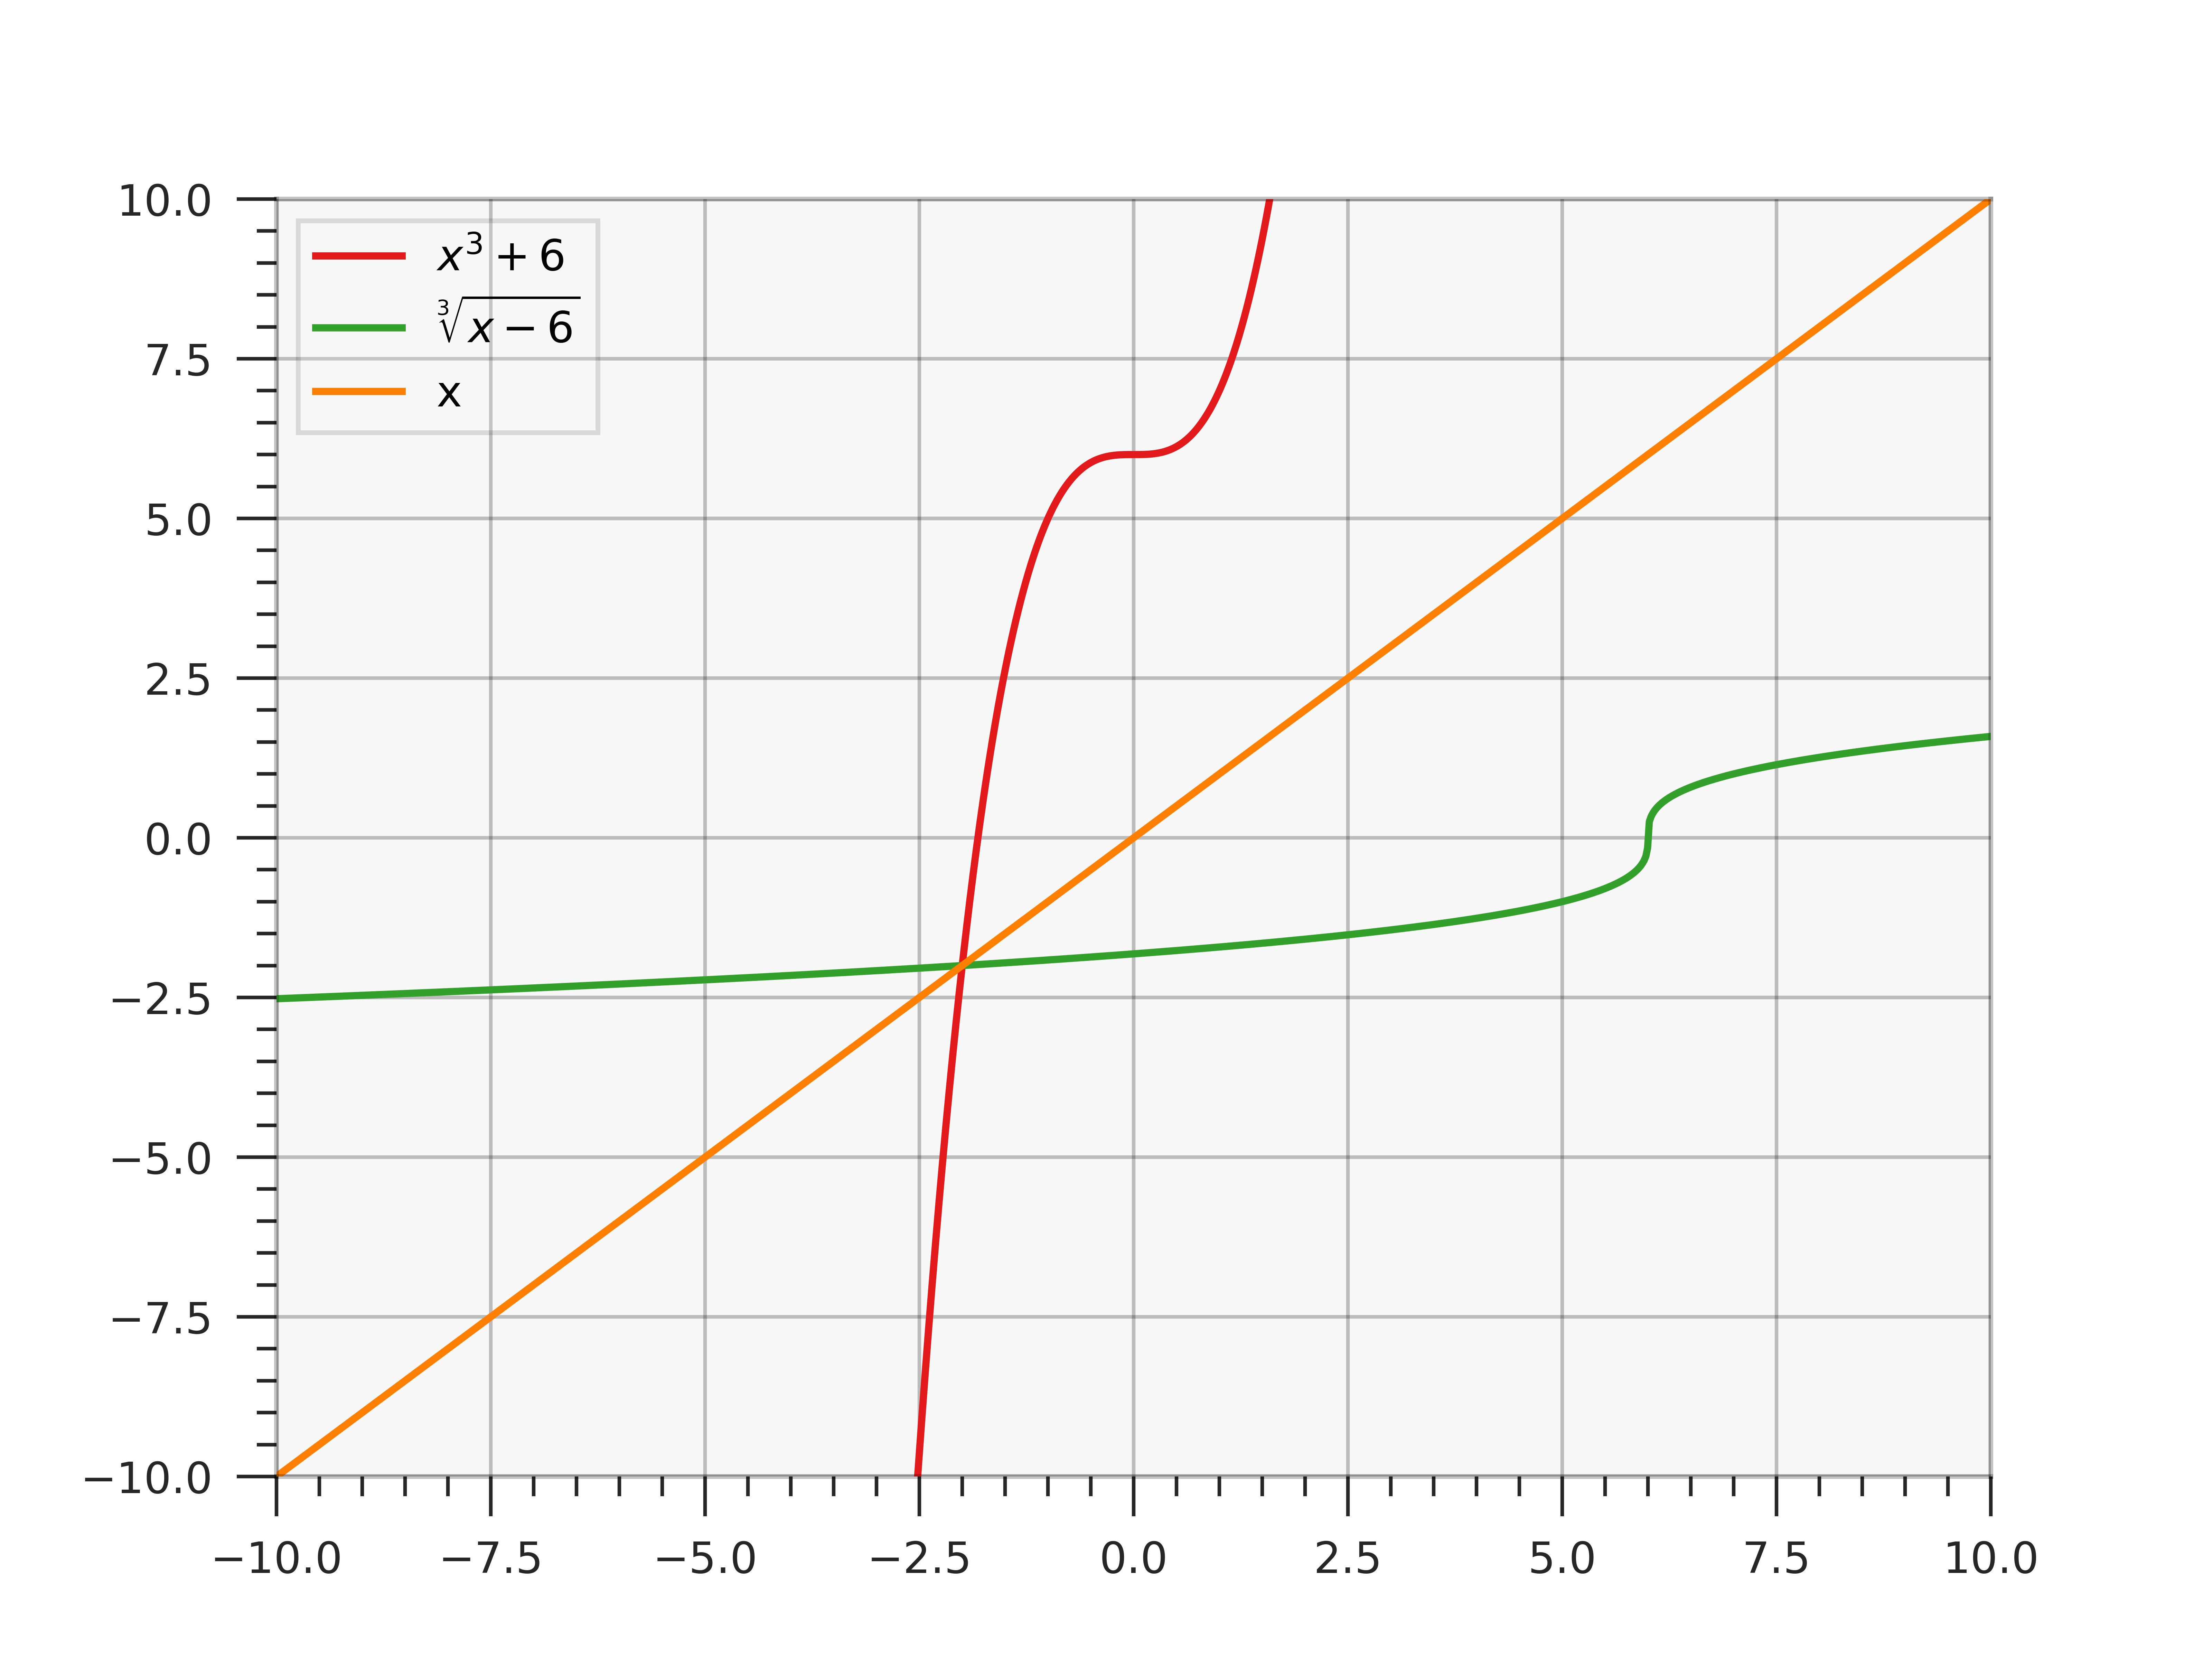
\includegraphics[width=12.5cm, height=10cm]{inverse_functions.png}
    \caption{Inverse Functions}
    \label{fig:fig1}
\end{figure}

This relation between inverse functions will be true for any $f(x)$ and $f^{-1}(x)$.
Even with functions that are not one-to-one, there will be this symmetry for some interval where the function does happen to be one-to-one.
For instance, the function $\sin(x)$ is mirrored with $\arcsin(x)$ in the interval $[-\pi, \pi]$, before the function repeats its $y$ values.

\end{document}